% Activate the following line by filling in the right side. If for example the name of the root file is Main.tex, write
% "...root = Main.tex" if the chapter file is in the same directory, and "...root = ../Main.tex" if the chapter is in a subdirectory.
 
%!TEX root = TNTinderSee.tex 
%%%%%%%%%%%%%%%%%%%%%%%%%%%%%%% 80-Char line %%%%%%%%%%%%%%%%%%%%%%%%%%%%%%%%%%

\chapter{Ergebnisse}

\section{Auswertung der Multibeamdaten}

Im Geomar konnten wir die Rohdaten analysieren. Auch das Grid, wurde weiter verfeinert, von 25cm$^2$ auf 10cm$^2$. 
Wir löschten fehlerhafte Daten, erstellten eine 3D-Karte des gescannten Gebiets und erzeugten ein sogenanntes \glqq Backscatter\grqq . 
Das Backscatter umfasst weniger die Tiefe des Gebiets, als die empfangene Lautstärke unserer Signale. 
Diese Lautstärke wird von der Tiefe des Gebiets und vor allem von der Beschaffenheit des Bodens bestimmt.

Generell kann man sagen, das, je härter der Boden ist, desto stärker die Schallwellen reflektiert werden. 
Auf der Backscatter-Karte wird diese Lautstärke veranschaulicht und man kann die Art des Bodens bestimmen.
Auch Munition würde auf dieser Karte stark auffallen, da Sie die Schallwellen stark reflektiert und so 
auf der Karte hell aufleuchten würde. Auf der von uns erzeugten Karte erkennt man die Seegraswiesen in der Nähe der Insel Vilm an ihrer geringen Reflektion.

\subsubsection{Fazit der optischen Multibeamauswertung}
Große Bruchstücke der Schuten oder herumliegende Munition konnten wir auf dem Multibeam keine erkennen und auch mit dem Tauchroboter stellten sich verdächtige Erhebungen als ungefährlich heraus. \\

\section{Optische Auswertung der ROV-Bilder}
\subsection{Identifikation von Munition}
Für den Hauptteil unserer Forschung, welche sich mit der Suche nach ehemaliger Kriegsmunition und der daraus folgende Umweltbelastung durch sprengstofftypischen Verbindungen beschäftigt,
hatte das ROV die Aufgabe die im Untersuchungsgebiet vermuteten Munitionsreste zu verifizieren. 
Im Jahre 1945 soll der Fißnowkahn Nr. 139 , unter Aufsicht des Russischen Militärs ca. 90 Tonnen Kriegsmunition zu versenken, hierbei kam es tragischwerweise zwischen Vilm und Lauerbach zu einer Explosion und die Bruchstücke des Kahns versanken mit der zu entladenden Munition im Gewässer vor der Insel Vilm.
Mithilfe des Multibeams haben wir vor Vilm lediglich zwei kleinere auffälige Objekte entdeckt, welche wir durch den ROV genauer betrachten konnten. Die auffälligere Stelle bestand auf dem Multibeam aus einem ca. 4m langen Objekt mit einem Durchmesser von einem Meter, was von der Größe eine Grundmine hätte sein können.
Nach der Inspektion durch den ROV hat sich zum Glück herausgestellt, das sich das Objekt nur um eine, vermutlich durch ein Anker entstandene, Rille mit einem Stahlseil darin handelt, und somit keine Gefahr davon ausging.
An der zweiten auffälligen Stelle haben wir beim Tauchen mit dem ROV nichts finden könne, vermutlich, weil wir hier besonders mit den o.g. Problemen zu kämpfen hatten. 

\subsubsection{Versuch einer 3D-Modellierung}
Eins unserer Ziele war, mit den oben gewonnenen Bilddaten ein 3D-Modell zu erstellen. Dazu wird das Kameravideo in Einzelbilder zerlegt und mit der Software \emph{Metashape} durch ein photogrammetrisches Verfahren ein 3D-Model erstellt. 
Nach dem Extrahieren der einzelnen Bilder und dem Import nach Metashape, mussten wir Feststellen, dass sich aus den relativ trüben Bildern keine hinreichend genauen Kameraperspektiven ableiten ließen, trotz einiger Tricks und Optimierung der entsprechenden Daten mit Hilfe von \emph{Yifan Song}, einem Spezialisten für Photogrammetrie am Geomar. So konnte Metashape leider kein 3D-Model erstellen.
Yifan Song wies uns darauf hin, dass die Software vor allem aufgrund der hohen \emph{Bewegungsunschärfe} und der ungünstigen Perspektive, resultierend aus Art der Kameraufhängung und der schlechten Unterwassersicht, Probleme hatte. 
Als Optimierung für unsere nächste Photogrammetrie mit dem ROV haben wir beschlossen, dass wir eine andere Kamera höherer Lichtempfindlichkeit und Bildfrequenz verbauen werden, um den Motion Blur zu reduzieren. Diese soll senkrecht auf den Boden und auf das Objekt gerichtet ist, so dass die einzelnen Bilder eine höhere Überlappung mit auffälligen Bildpunkten haben.
\\

Der zweite Teil der Bildauswertung bestand darin herauszufinden, ob man mithilfe des Multibeams Seegraswiesen und Makrophyten kartieren kann. Hierbei haben wir die Strukturen in der Multibeamkarte mit dem wahren Untergrund durch das ROV bestimmt.
Bei der Rückstrahlung der hydroakustischen Wellen und somit der Struktur der Multibeamkarte spielt einerseits die Flora des Untergrunds eine Rolle, andererseits auch die Art des Sediments.
Aus diesem Grund haben wir einen eigenen Aufsatz für das ROV entwickelt und mit dem 3D-Drucker gedruckt der es uns erlaubt, gezielt Sedimentproben zu nehmen, um nach der Analyse der Korngröße auf das Rückstrahlvehalten schließen zu können.
Hierbei ist uns aufgefallen das in der Nähe der Seegraswiesen und Makrophyten das Sediment tendenziell feiner ist und in den Arealen ohne dieser Flora eher gröber.
Um den genauen Verlauf der Flora hin zu den Seegraswiesen mit der Multibeamkarte vergleichen zu können wollten wir ebenfalls ein 3D-Modell erstellen, hierbei hatten wir jedoch die gleichen Probleme wie bei der Photogrammertrie der aufälligen Objekte, wodurch wir auch mit diesem 3D-Modell vorerst gescheitert sind.

\subsubsection{Fazit der optischen Auswertung}
Obwohl im Endeffekt nicht viel von dem, was wir mit dem ROV vor hatten, wirklich geglückt ist, haben wir sowohl beim Operating des ROVs, als auch in Hinsicht der Datenauswertungen viel Erfahrungen sammeln können. Und die vermeintliche Grundmine konnte mit Hilfe des ROV noch vor Ort als ungefährliche Ankerfurche identifiziert werden.

\section{Wasseranalyse}
Auf der Abbildung 3.2. sieht man, wie die Nachweise der Verbindungen HMX, RDX, TNT und ADTNT (von oben nach unten) hätten aussehen sollen. In unseren Messergebnissen (Abb. 3.1. zeigt beispielhaft Messpunkt W1, es sahen aber alle ähnlich aus), sind an den erwarteten Zeit keinerlei signifikante Spitzen zu erkennen. Wir konnten, für uns durchaus etwas überraschend, keinerlei sprengstofftypische Verbindungen nachweisen.

\begin{figure}[htb!]
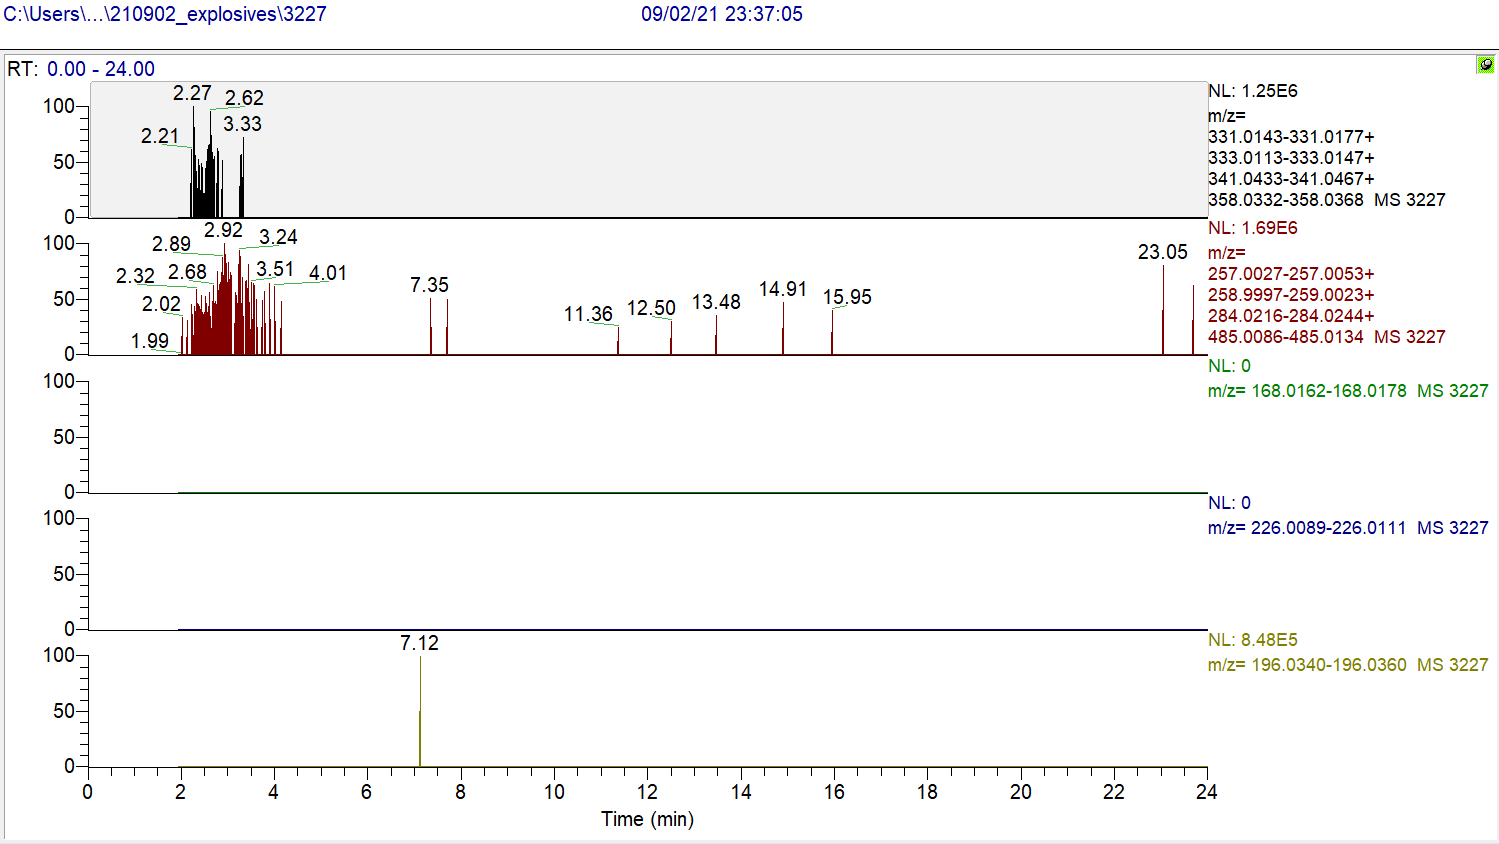
\includegraphics[height=\textheight,%
                   width=\textwidth,%
                   keepaspectratio]{Bilder/Explosives_3227_SampleW1.PNG}
\caption{Chromatografieergebnis mit Focus auf sprengstofftypischen Verbindungen. HMX (schwarz), RDX (grün), TNT (blau), ADNT (gelb)}
\end{figure}

\begin{figure}[htb!]
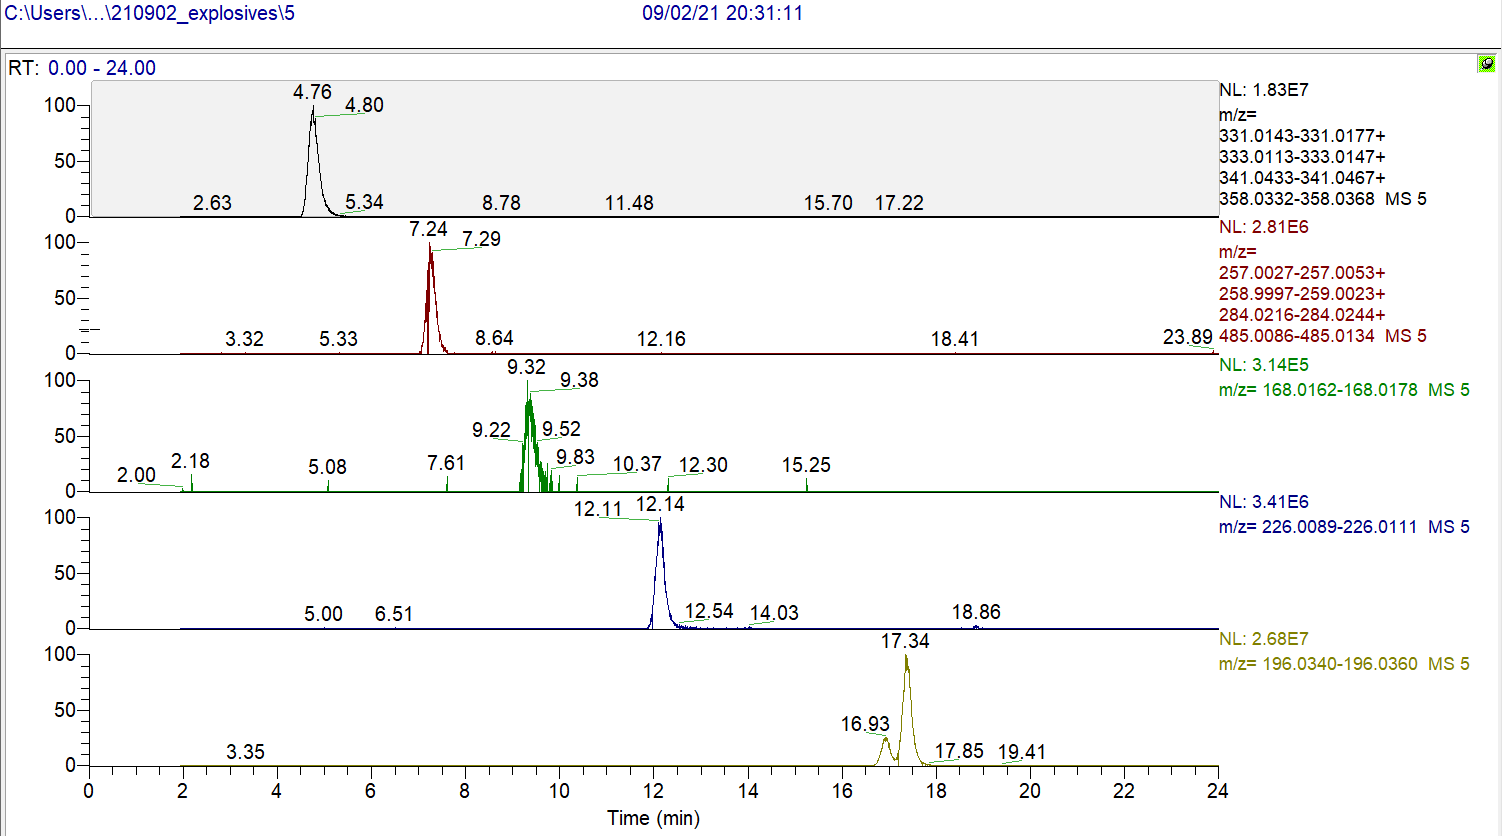
\includegraphics[height=\textheight,%
                   width=\textwidth,%
                   keepaspectratio]{Bilder/Explosives_5ppb.PNG}
\caption{Vergleichende Standardwerte bei Nachweis sprengstofftypischer Verbindungen}
\end{figure}

\section{Sedimentanalyse}
Die Sedimentanalyse haben wir, weil sie aufwändig ist, abhängig von den Ergebnissen der Wasseranalyse gemacht. Und weil dessen Ergebnisse keinerlei STVs andeuten, (bisher noch) nicht durchgeführt.

\section{Diskussion der Ergebnisse}
Obwohl eine Schute mit 90 Tonnen Munition im Untersuchungsgebiet gesunken ist, konnten wir weder optisch Munitionsreste ausmachen, als auch keine sprengstofftypischen Rückstände im Wasser nachweisen. Zum derzeitigen Zeitpunkt haben wir die Bodenproben noch nicht analysiert, wir halten es aber für eher unwahrscheinlich, hier noch Munitionsnachweise zu finden.
\\
Nach diesen Ergebnissen können wir Entwarnung geben: Das von uns abgesuchte Gebiet ist offensichtlich unbelastet. Ein solches Ergebnis ist zwar unspektakulär, aber erleichternd. Wieso 
unsere Proben keine Spuren von Sprengstoffen oder deren Zerfallsprodukten 
enthalten ist eine andere Frage. Wir vermuten, dass die gesunkende Munition in späteren Jahren wieder geborgen wurde und wir deshalb keine Reste mehr fanden.
Eventuell verbleibende Munitionsreste könnten von der Biomasse vor Ort aufgenommen worden sein, diese musste für die Ionenchromatografie nämlich aus den Proben gefiltert werden, so dass wir deshalb keine Rückstände hätten nachweisen können. \\ 
Um diese Frage zu beantworten wäre eine andere Messmethode und eine erneute Forschungsfahrt nötig.